% Figure 1: conceptual overview of CEL (one ledger, two modes).
% Build: pdflatex fig1_overview.tex  ->  fig1_overview.pdf (included by main.tex).
% Shown symbolically: the standard (eps0, p0*) is the user's dial and d*, B* are derived from it.
% Paper default (sprt_posterior.py): k1=3, (eps0, p0*)=(0.05, 0.8) -> d*=9, eps(9,9)=0.042.
\documentclass[tikz,border=2pt]{standalone}
\usepackage{amsmath,amssymb,pifont}
\usepackage[scaled=0.92]{helvet}
\renewcommand{\familydefault}{\sfdefault}
\usetikzlibrary{arrows.meta,calc,positioning,decorations.pathreplacing,backgrounds}

% Okabe-Ito palette (colour-blind safe)
\definecolor{agree}{HTML}{009E73}
\definecolor{fail}{HTML}{D55E00}
\definecolor{probe}{HTML}{0072B2}
\definecolor{other}{HTML}{CC79A7}
\definecolor{gen}{HTML}{999999}
\definecolor{ink}{HTML}{222222}

\newcommand{\cb}[1]{{\ding{\numexpr181+#1\relax}}}
\newcommand{\ok}{\ding{51}}
\newcommand{\no}{\ding{55}}

\tikzset{
  cell/.style={minimum size=0.36cm,inner sep=0,draw=white,line width=0.6pt,font=\scriptsize\bfseries,text=white},
  ghost/.style={minimum size=0.36cm,inner sep=0,draw=gen!60,dashed,line width=0.4pt},
  panel/.style={rounded corners=3pt,draw=gen!50,line width=0.5pt,fill=gray!3},
  box/.style={rounded corners=2pt,draw=ink!70,line width=0.5pt,fill=white,align=left,inner sep=3pt,font=\scriptsize},
  title/.style={font=\footnotesize\bfseries,anchor=north west,text=ink},
  note/.style={font=\scriptsize,text=ink!80,align=left},
  brace/.style={decorate,decoration={brace,amplitude=3pt,raise=1pt},line width=0.5pt,ink!70},
  badge/.style={circle,fill=ink,text=white,font=\scriptsize\bfseries,inner sep=0pt,minimum size=0.36cm},
  flow/.style={-{Stealth[length=5pt]},line width=0.8pt,ink!70},
}

% one ledger cell: \C{x}{y}{colour}{label}
\newcommand{\C}[4]{\node[cell,fill=#3] at (#1,#2) {#4};}

\begin{document}
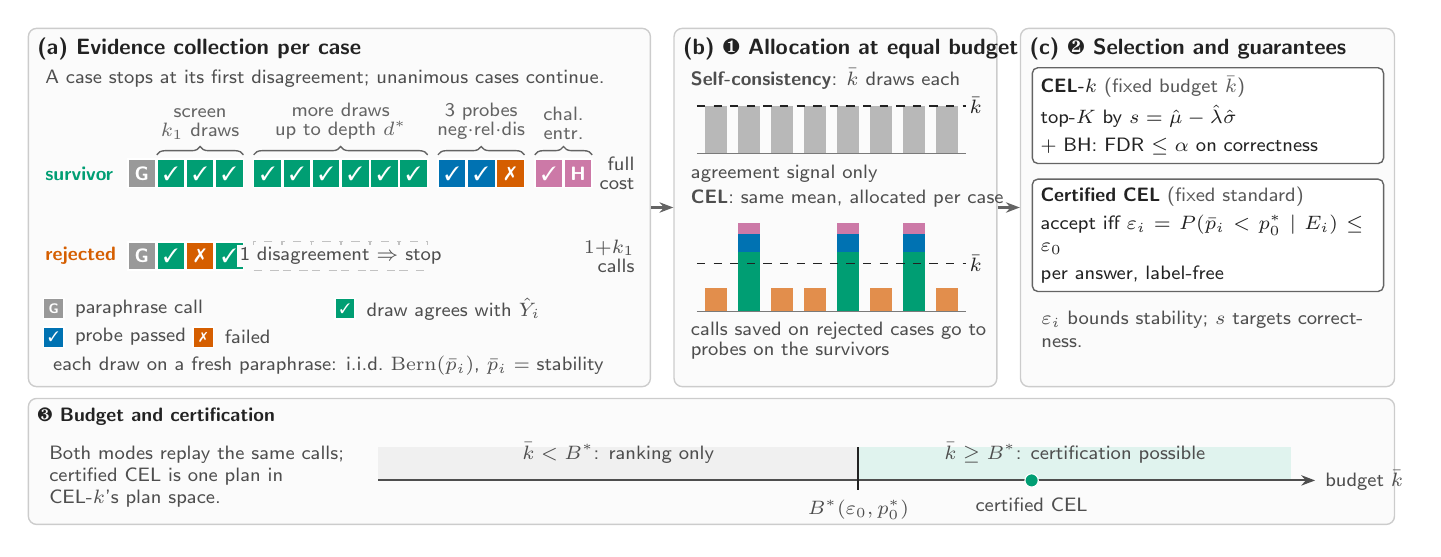
\begin{tikzpicture}[x=1cm,y=1cm,font=\scriptsize,text=ink]

% ======================= (a) the evidence ledger =========================
\def\s{0.37}  % cell pitch
\def\yA{0}    % survivor row
\def\yB{-1.05} % eliminated row
\def\xo{1.3} % first cell
\begin{scope}[on background layer]
  \node[panel,minimum width=7.9cm,minimum height=4.55cm,anchor=north west] (PA) at (-0.15,1.85) {};
\end{scope}
\node[title] at (PA.north west) {(a) Evidence collection per case};
\node[note,anchor=north west] at ($(PA.north west)+(0.1,-0.42)$)
  {A case stops at its first disagreement; unanimous cases continue.};

% survivor row: gen | 3 screen draws | 6 draws | 3 probes | challenge | entropy
\node[note,anchor=west] at (-0.05,\yA) {\textcolor{agree}{\textbf{survivor}}};
\C{\xo}{\yA}{gen}{G}
\foreach \k in {1,2,3} {\C{\xo+\k*\s}{\yA}{agree}{\ok}}
\foreach \k in {4,...,9} {\C{\xo+\k*\s+0.12}{\yA}{agree}{\ok}}
\C{\xo+10*\s+0.24}{\yA}{probe}{\ok}
\C{\xo+11*\s+0.24}{\yA}{probe}{\ok}
\C{\xo+12*\s+0.24}{\yA}{fail}{\no}
\C{\xo+13*\s+0.36}{\yA}{other}{\ok}
\C{\xo+14*\s+0.36}{\yA}{other}{H}
\node[note,anchor=east,align=right] at (7.68,\yA) {full\\[-1pt]cost};

% braces over the survivor row
\draw[brace] (\xo+1*\s-0.18,\yA+0.2) -- node[above=3pt,align=center]{screen\\[-1pt]$k_1$ draws} (\xo+3*\s+0.18,\yA+0.2);
\draw[brace] (\xo+4*\s+0.12-0.18,\yA+0.2) -- node[above=3pt,align=center]{more draws\\[-1pt]up to depth $d^\ast$} (\xo+9*\s+0.12+0.18,\yA+0.2);
\draw[brace] (\xo+10*\s+0.24-0.18,\yA+0.2) -- node[above=3pt,align=center]{3 probes\\[-1pt]neg$\cdot$rel$\cdot$dis} (\xo+12*\s+0.24+0.18,\yA+0.2);
\draw[brace] (\xo+13*\s+0.36-0.18,\yA+0.2) -- node[above=3pt,align=center]{chal.\\[-1pt]entr.} (\xo+14*\s+0.36+0.18,\yA+0.2);

% eliminated row: gen | screen with a disagreement | stop
\node[note,anchor=west] at (-0.05,\yB) {\textcolor{fail}{\textbf{rejected}}};
\C{\xo}{\yB}{gen}{G}
\C{\xo+1*\s}{\yB}{agree}{\ok}
\C{\xo+2*\s}{\yB}{fail}{\no}
\C{\xo+3*\s}{\yB}{agree}{\ok}
\foreach \k in {4,...,9} {\node[ghost] at (\xo+\k*\s+0.12,\yB) {};}
\node[note,fill=gray!3,inner sep=1pt] at (\xo+6.5*\s+0.12,\yB) {1 disagreement $\Rightarrow$ stop};
\node[note,anchor=east,align=right] at (7.68,\yB) {$1{+}k_1$\\[-1pt]calls};


% legend
\begin{scope}[shift={(0.05,-1.72)}]
  \node[cell,fill=gen,minimum size=0.26cm,font=\tiny\bfseries] at (0.13,0) {G};
  \node[note,anchor=west] at (0.28,0) {paraphrase call};
  \node[cell,fill=agree,minimum size=0.26cm,font=\tiny] at (3.83,0) {\ok};
  \node[note,anchor=west] at (3.98,0) {draw agrees with $\hat Y_i$};
  \node[cell,fill=probe,minimum size=0.26cm,font=\tiny] at (0.13,-0.36) {\ok};
  \node[note,anchor=west] at (0.28,-0.36) {probe passed};
  \node[cell,fill=fail,minimum size=0.26cm,font=\tiny] at (2.03,-0.36) {\no};
  \node[note,anchor=west] at (2.18,-0.36) {failed};
  \node[note,anchor=west] at (0.0,-0.72) {each draw on a fresh paraphrase: i.i.d.\ $\mathrm{Bern}(\bar p_i)$, $\bar p_i$ = stability};
\end{scope}

% ======================= (b) matched budget, reallocated (contribution 1) =========
% Illustrative: 8 cases; CEL rejects 5 at 1+k1 = 4 calls and spends 15 on 3 survivors,
% mean 65/8 = 8.1, the same as self-consistency at 8 draws each.
\begin{scope}[on background layer]
  \node[panel,minimum width=4.1cm,minimum height=4.55cm,anchor=north west] (PB) at (8.05,1.85) {};
\end{scope}
\node[title] at (PB.north west) {(b)~\cb{1}~Allocation at equal budget};
\def\u{0.075}  % cm per call
\def\bx{8.45}\def\bp{0.42}\def\bw{0.28}
% self-consistency
\def\ya{0.25}
\node[note,anchor=west] at (8.15,1.2) {\textbf{Self-consistency}: $\bar k$ draws each};
\foreach \c in {0,...,7} {\fill[gen!70] (\bx+\c*\bp,\ya) rectangle ++(\bw,8*\u);}
\draw[ink!60,line width=0.4pt] (\bx-0.1,\ya) -- (\bx+7*\bp+\bw+0.1,\ya);
\node[note,anchor=north west] at (8.15,\ya-0.02) {agreement signal only};
% CEL
\def\yb{-1.75}
\node[note,anchor=west] at (8.15,-0.32) {\textbf{CEL}: same mean, allocated per case};
\foreach \c/\surv in {0/0,1/1,2/0,3/0,4/1,5/0,6/1,7/0} {
  \ifnum\surv=1
    \fill[agree] (\bx+\c*\bp,\yb) rectangle ++(\bw,10*\u);
    \fill[probe] (\bx+\c*\bp,\yb+10*\u) rectangle ++(\bw,3*\u);
    \fill[other] (\bx+\c*\bp,\yb+13*\u) rectangle ++(\bw,2*\u);
  \else
    \fill[fail!70] (\bx+\c*\bp,\yb) rectangle ++(\bw,4*\u);
  \fi}
\draw[ink!60,line width=0.4pt] (\bx-0.1,\yb) -- (\bx+7*\bp+\bw+0.1,\yb);
\foreach \y in {\ya,\yb} {\draw[dashed,ink,line width=0.5pt] (\bx-0.1,\y+8.1*\u) -- (\bx+7*\bp+\bw+0.1,\y+8.1*\u) node[right,inner sep=1pt,font=\scriptsize] {$\bar k$};}
\node[note,anchor=north west] at (8.15,\yb-0.02) {calls saved on rejected cases go to\\[-1pt]probes on the survivors};

% ======================= (c) one ledger, two guarantees (contribution 2) ==========
\begin{scope}[on background layer]
  \node[panel,minimum width=4.75cm,minimum height=4.55cm,anchor=north west] (PC) at (12.45,1.85) {};
\end{scope}
\node[title] at (PC.north west) {(c)~\cb{2}~Selection and guarantees};

\node[box,anchor=north west,text width=4.25cm] (MK) at ($(PC.north west)+(0.15,-0.5)$) {%
  \textbf{CEL-$k$} {\color{ink!75}(fixed budget $\bar k$)}\\[2pt]
  top-$K$ by $s=\hat\mu-\hat\lambda\hat\sigma$\\[2pt]
  + BH: FDR $\le\alpha$ on correctness};

\node[box,anchor=north west,text width=4.25cm] (MC) at ($(MK.south west)+(0,-0.18)$) {%
  \textbf{Certified CEL} {\color{ink!75}(fixed standard)}\\[2pt]
  accept iff $\varepsilon_i=P(\bar p_i<p_0^\ast\mid E_i)\le\varepsilon_0$\\[2pt]
  per answer, label-free};

\node[note,anchor=north west,text width=4.3cm] at ($(MC.south west)+(0,-0.12)$)
  {$\varepsilon_i$ bounds stability; $s$ targets correctness.};

% arrows between panels
\draw[flow] (PA.east) -- (PB.west);
\draw[flow] (PB.east) -- (PC.west);

% ======================= budget axis (bottom strip) ======================
\def\yb{-3.6}
\begin{scope}[on background layer]
  \node[panel,minimum width=17.35cm,minimum height=1.6cm,anchor=north west] (PD) at (-0.15,\yb+0.75) {};
\end{scope}
\node[title,font=\scriptsize\bfseries] at (PD.north west) {\cb{3}~Budget and certification};
\node[note,anchor=north east] at ($(PD.north east)+(-0.15,-0.08)$) {};
\def\xl{4.3}\def\xr{15.9}\def\xB{10.4}\def\xC{12.6}
\fill[gray!12] (\xl,\yb-0.3) rectangle (\xB,\yb+0.12);
\fill[agree!12] (\xB,\yb-0.3) rectangle (\xr,\yb+0.12);
\draw[-{Stealth[length=5pt]},line width=0.7pt,ink!80] (\xl,\yb-0.3) -- (\xr+0.3,\yb-0.3) node[right,note] {budget $\bar k$};
\node[note,anchor=south] at ($(\xl,\yb-0.2)!0.5!(\xB,\yb-0.2)$) {$\bar k<B^\ast$: ranking only};
\node[note,anchor=south] at ($(\xB,\yb-0.2)!0.5!(\xr,\yb-0.2)$) {$\bar k\ge B^\ast$: certification possible};
\draw[line width=0.8pt,ink] (\xB,\yb-0.42) -- (\xB,\yb+0.12) node[above,inner sep=1pt,font=\scriptsize\bfseries] {};
\node[note,anchor=north] at (\xB,\yb-0.42) {$B^\ast(\varepsilon_0,p_0^\ast)$};
\node[circle,fill=agree,draw=white,inner sep=1.7pt] at (\xC,\yb-0.3) {};
\node[note,anchor=north] at (\xC,\yb-0.4) {certified CEL};
\node[note,anchor=west,text width=4.1cm] at (0.0,\yb-0.25) {Both modes replay the same calls;\\certified CEL is one plan in\\CEL-$k$'s plan space.};

\end{tikzpicture}
\end{document}
